%{{{ Formatierung

\documentclass[a4paper,10pt]{article}

\usepackage{physics_notetaking}

%%% dark red
%\definecolor{bg}{RGB}{60,47,47}
%\definecolor{fg}{RGB}{255,244,230}
%%% space grey
%\definecolor{bg}{RGB}{46,52,64}
%\definecolor{fg}{RGB}{216,222,233}
%%% purple
%\definecolor{bg}{RGB}{69,0,128}
%\definecolor{fg}{RGB}{237,237,222}
%\pagecolor{bg}
%\color{fg}

\newcommand{\td}{\,\text{d}}
\newcommand{\RN}[1]{\uppercase\expandafter{\romannumeral#1}}
\newcommand{\zz}{\mathrm{Z\kern-.3em\raise-0.5ex\hbox{Z} }}
\newcommand{\id}{1\kern-.258em1}

\newcommand\inlineeqno{\stepcounter{equation}\ {(\theequation)}}
\newcommand\inlineeqnoa{(\theequation.\text{a})}
\newcommand\inlineeqnob{(\theequation.\text{b})}
\newcommand\inlineeqnoc{(\theequation.\text{c})}

\newcommand\inlineeqnowo{\stepcounter{equation}\ {(\theequation)}}
\newcommand\inlineeqnowoa{\theequation.\text{a}}
\newcommand\inlineeqnowob{\theequation.\text{b}}
\newcommand\inlineeqnowoc{\theequation.\text{c}}

\renewcommand{\refname}{Source}
\renewcommand{\sfdefault}{phv}
%\renewcommand*\contentsname{Contents}

\newenvironment{Figure}
        {\par\medskip\noindent\minipage{\linewidth}}
        {\endminipage\par\medskip} % for multicols figures

\pagestyle{fancy}

\sloppy

\numberwithin{equation}{section}

%}}}

\begin{document}

%{{{ Titelseite

\begin{titlepage}
	\title{6 (2. Halbtag) $|$ Operationsverstärker}
	\author[1]{Angelo Brade\thanks{s72abrad@uni-bonn.de}}
	\author[1]{Jonas Wortmann\thanks{s02jwort@uni-bonn.de}}
	\affil{Rheinische Friedrich--Wilhemls Universität Bonn}
\end{titlepage}

\iffalse\title{}
\author{}\fi

\maketitle
\pagenumbering{gobble}

%}}}

\clearpage

%{{{ Inhaltsverzeichnis

\fancyhead[R]{\leftmark}
%\fancyhead[R]{\leftmark\\\rightmark}
\fancyhead[L]{\thepage}
\fancyfoot[C]{}

\tableofcontents

%}}}

\clearpage

%{{{

\pagenumbering{arabic}

\begin{multicols}{2}
	\sloppy

	\section{Introduction}
	In this experiment, 6 groups will constrcut 6 different circuits and connect them to one big circuit.
	The result will look like this.
	\begin{Figure}
		\centering
		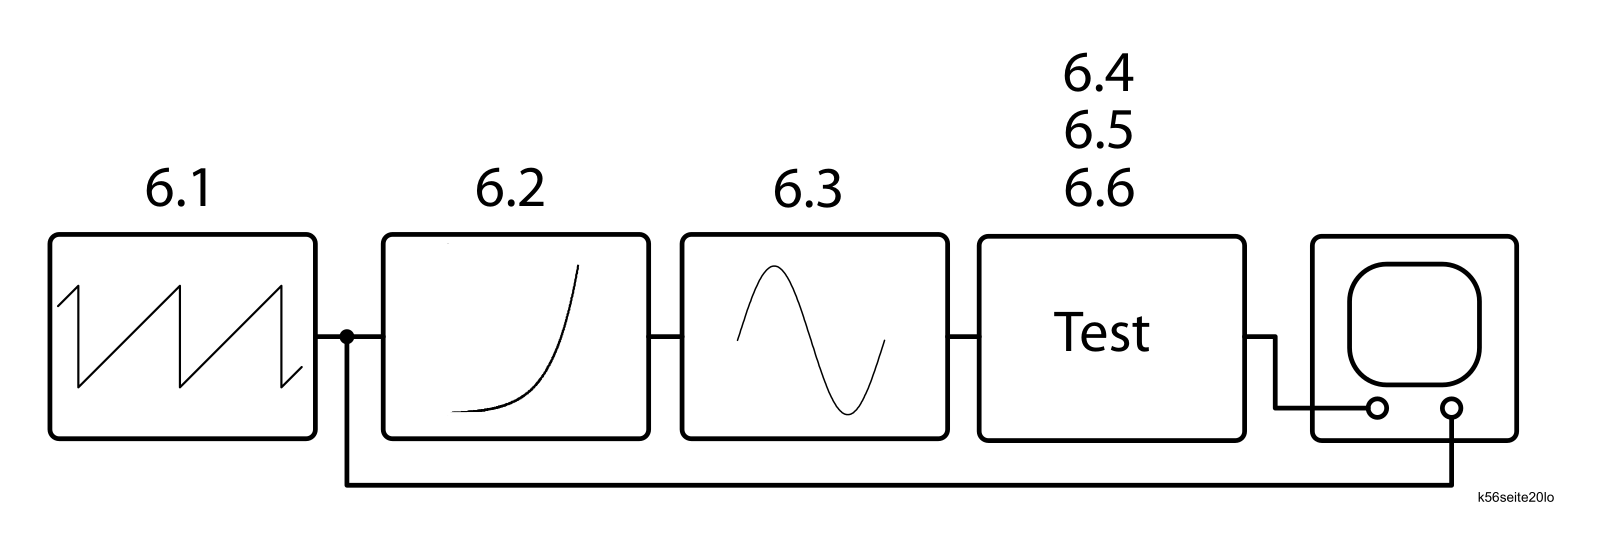
\includegraphics[width=0.7\textwidth]{result.png}
		\captionof{figure}{Circuit built from 6 individual smaller circuits; Abb. 6.14\cite{Praktikumsanleitung}}
	\end{Figure}
	\noindent This resulting circuit will show different usecases of the opamp, for example, demonstrate different configurations of high-- and lowpass filters as well as working as a resonanz amplifier.
        
	\section{Theory}
	The six different circtuis are
	\begin{enumerate}[label=\arabic*]
		\item Ramp generator:
		      The ramp generator will input a ramp signal to the whole circuit.
		      The signal will be generated via the astable multivibrator.
		      This circuit utilises a condensator which charges and discharges in a certain time interval.
		\item Exponentiator:
		      The inverting exponentiator has a very high input impedance compared to the non--inverting exponentiator, which makes it more suitable for this task.
		      \begin{Figure}
			      \centering
			      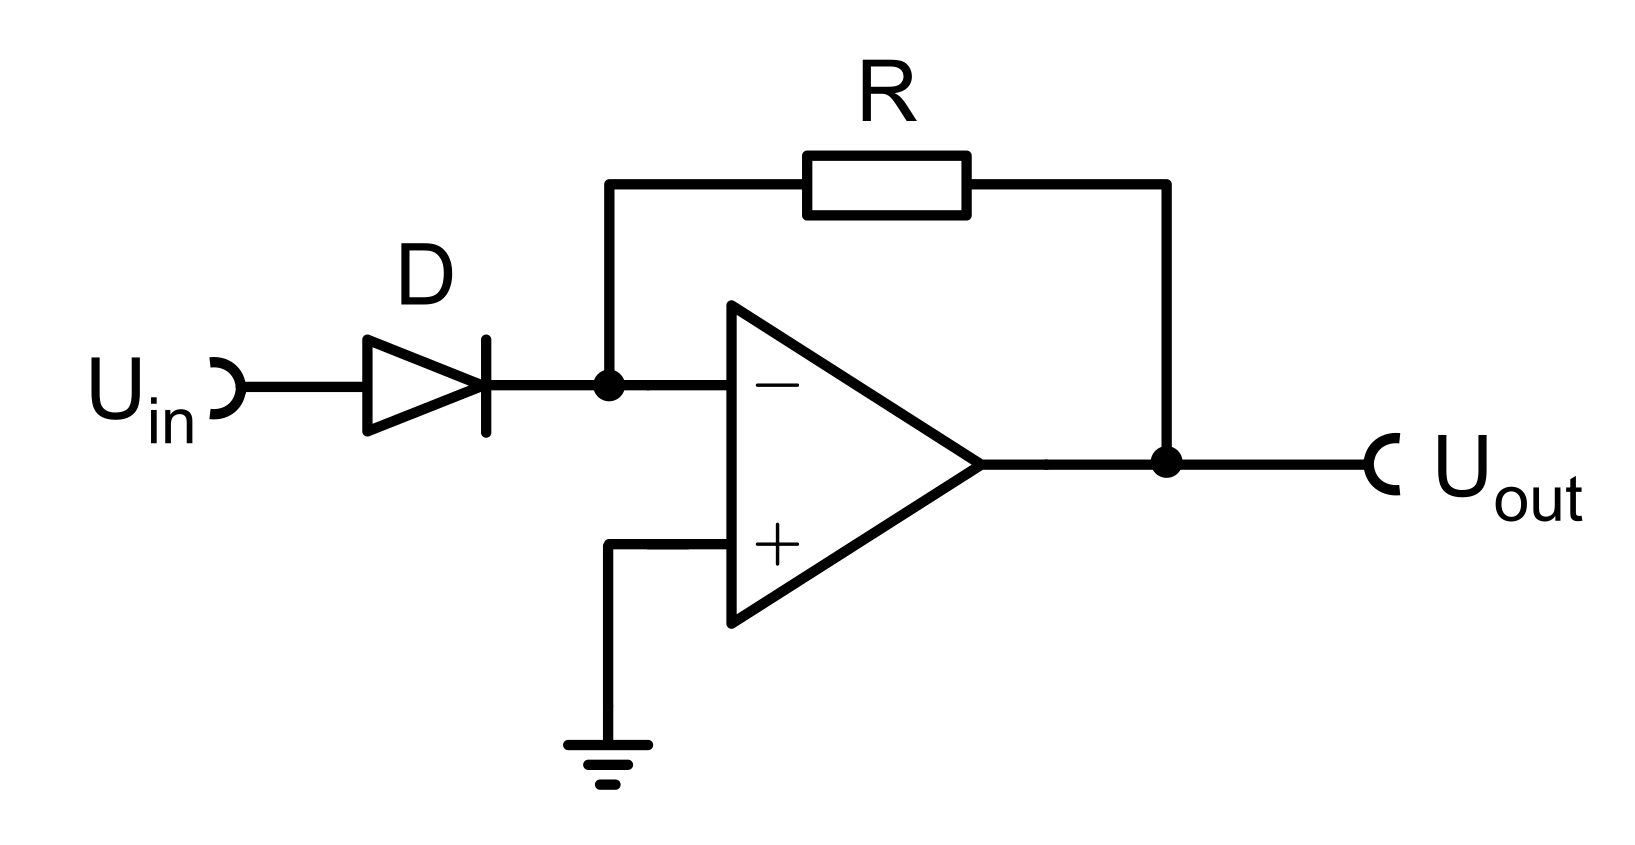
\includegraphics[width=0.6\textwidth]{inverting_exp.png}
			      \captionof{figure}{Inverting exponentiator; Abb.\ 6.4\cite{Praktikumsanleitung}}
			      \label{fig:invexpo}
		      \end{Figure}
		\item Voltage--frequency changer:
		      This circuit proudces a triangle signal with constant amplitude by charging and discharging a capacitor.
		      The current is proportional to the input voltage.
		      \begin{Figure}
			      \centering
			      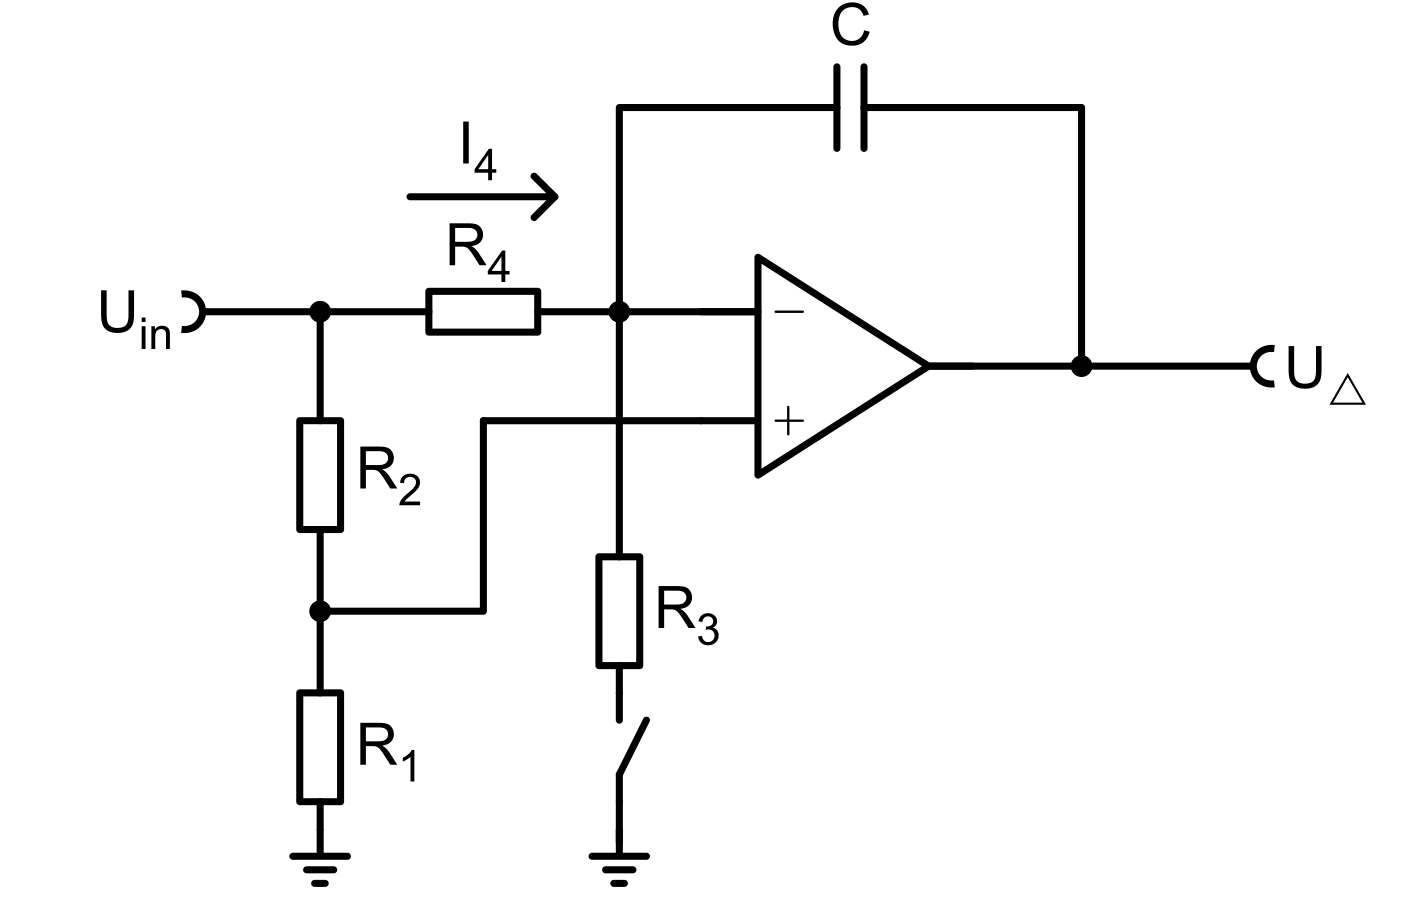
\includegraphics[width=0.6\textwidth]{reversible_integrator.png}
			      \captionof{figure}{Reversible integrator; Abb.\ 6.6\cite{Praktikumsanleitung}}
		      \end{Figure}
		      If the switch is open, the circuit behaves like a normal integrator and produces a constant decreasing output signal with current $I_4$.
		      If the switch is closed, a current across $R_3$ flows into the circuit which changes the sign of $I_4$ because both currents add.
		      This results in a constant increasing otuput signal.
		      For later use, the triangle signal will be modified into a sinosoidal signal.
		\item High-- and low--pass:
		      For this circuit a third order low--pass is used, by connecting three low--passes in a row all seperated by an opamp with $\nu =1$.
		      \begin{Figure}
			      \centering
			      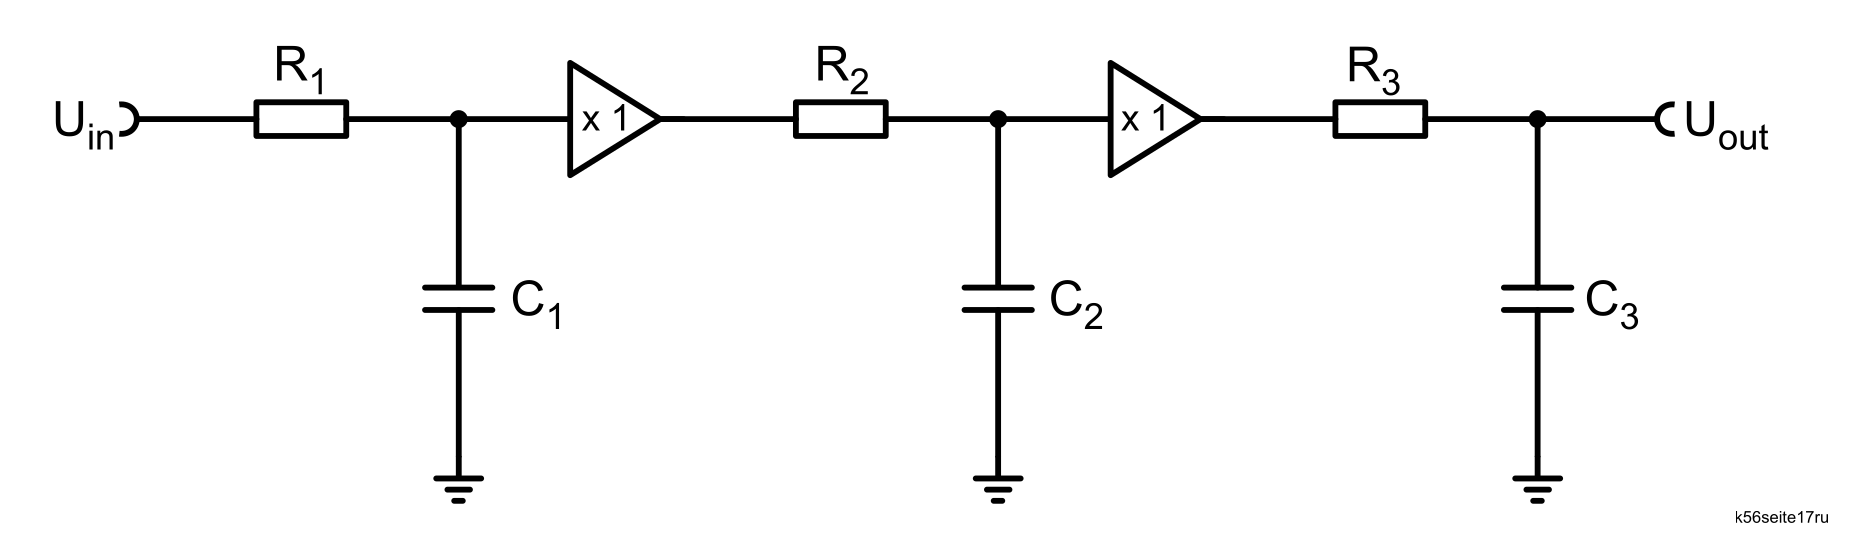
\includegraphics[width=0.6\textwidth]{lowpass_third_order.png}
			      \captionof{figure}{Third order low--pass; Abb.\ 6.10\cite{Praktikumsanleitung}}
		      \end{Figure}
		      In this configuration, their frequency response is multiplied.
		\item Band--elimination filter and resonance amplifier:
		      In this circuit a signal is sent through two low-- and high--passes connected in row.
		      The two output signals are then added via an opamp.
		      This results in a band--elimination filter.
		      \begin{Figure}
			      \centering
			      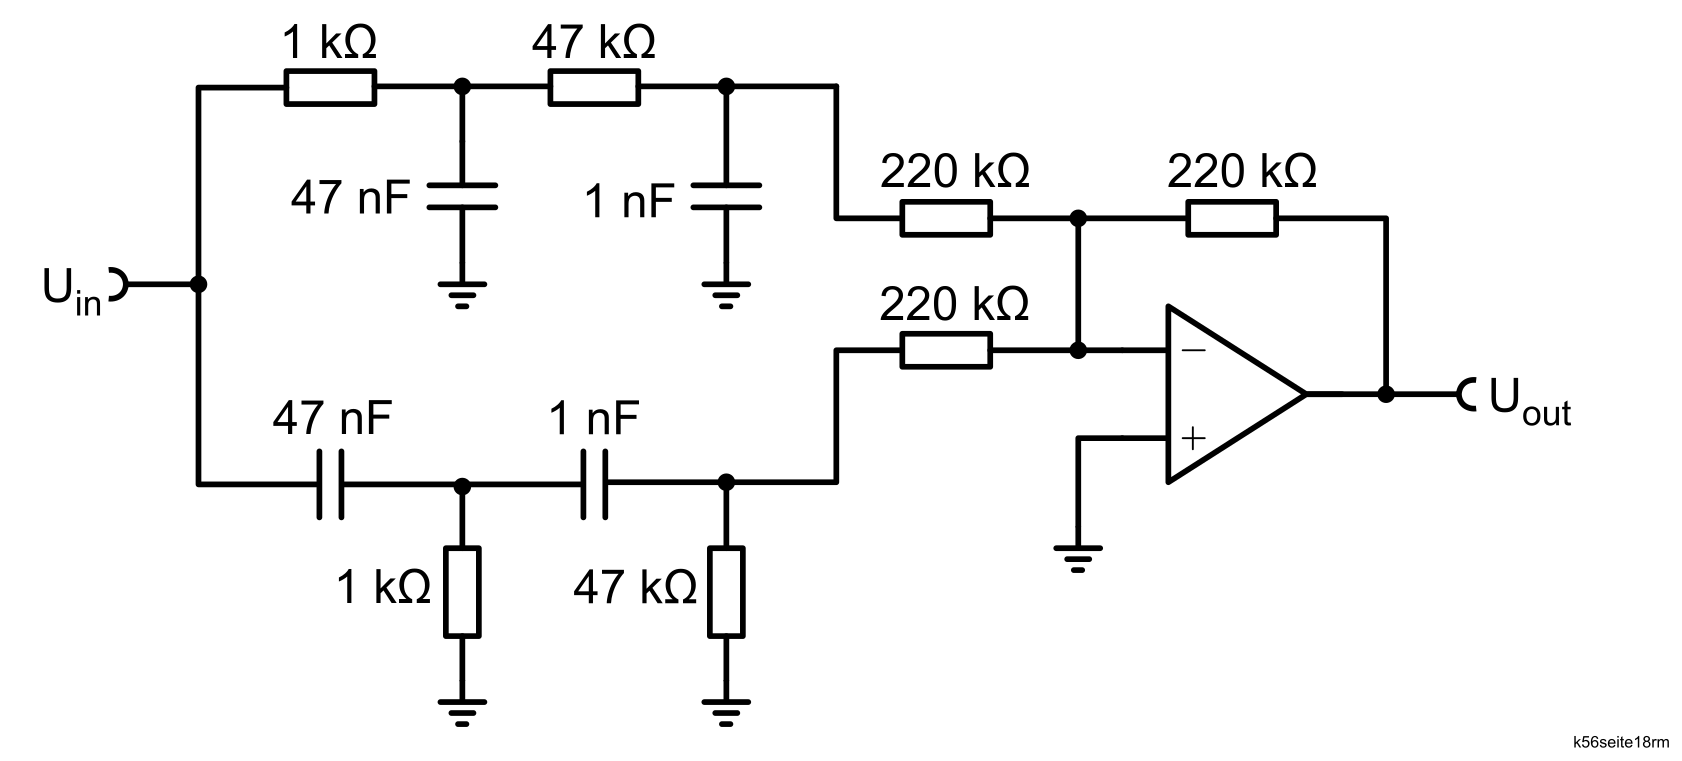
\includegraphics[width=0.6\textwidth]{band_elimination_filter.png}
			      \captionof{figure}{Band--elimination filter; Abb.\ 6.12\cite{Praktikumsanleitung}}
		      \end{Figure}
		\item Band--pass:
		      The last part is a band--pass.
		      \begin{Figure}
			      \centering
			      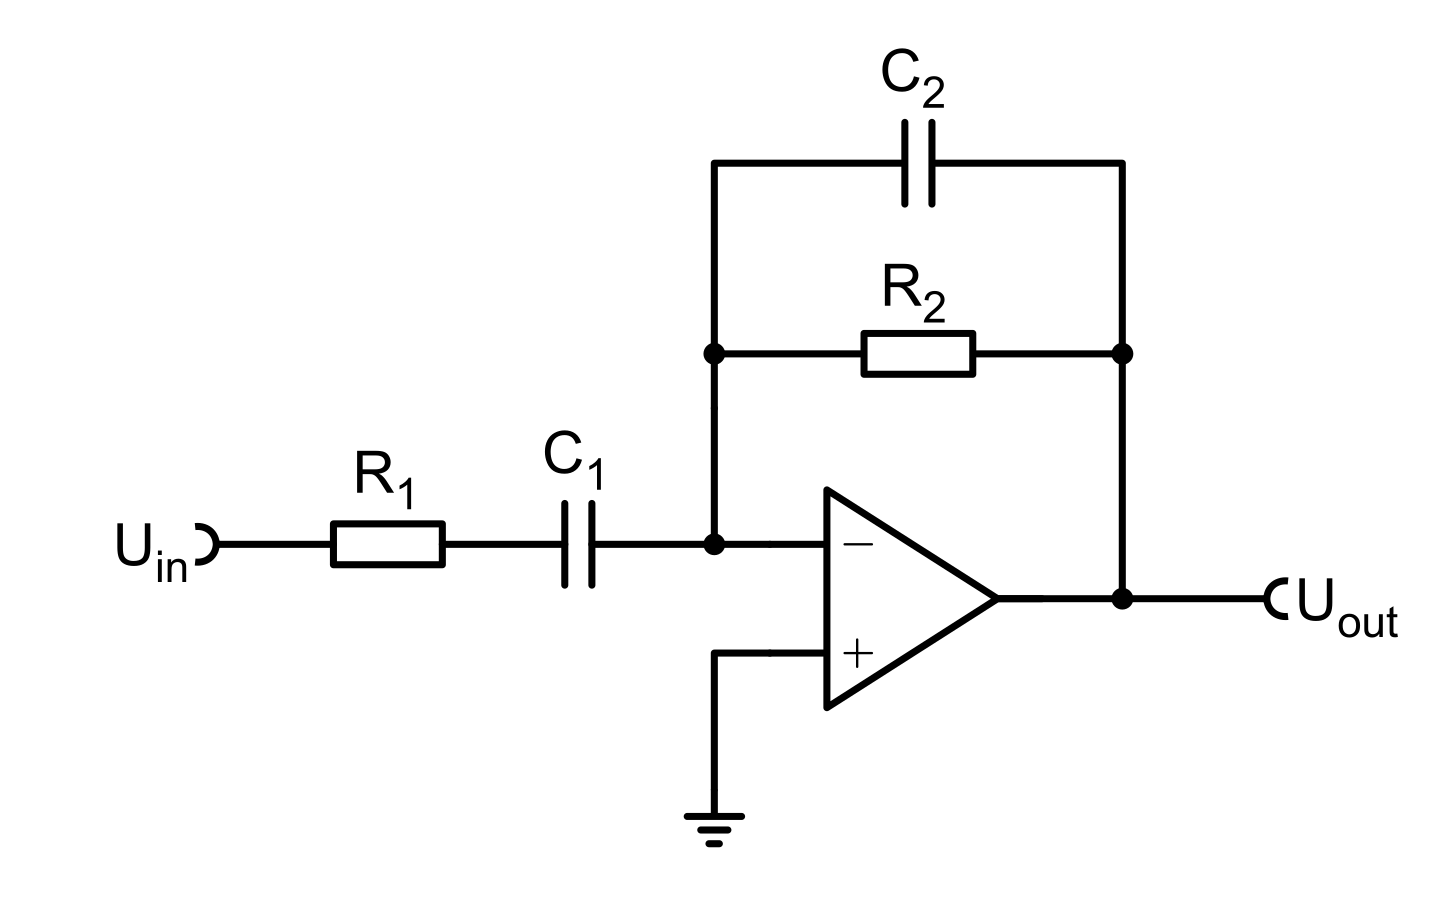
\includegraphics[width=0.6\textwidth]{bandpass.png}
			      \captionof{figure}{Band--pass; Abb.\ 6.13\cite{Praktikumsanleitung}}
		      \end{Figure}
	\end{enumerate}

	\clearpage
	\section{Analysis}
	\subsection{Inverting Exponentiater}
	Firstly we have a look at the inverting exponentiater shown in fig. \ref{fig:invexpo}. From here we see that $U_{-}=0$, since it is connected to ground. Furthermore we know from the first golden rule, that $U_{-}=U_{+}$, so $U_{+}$ is also 0. The second golden rule sais $I_{+}=I_{-}=0$. To calculate the current through the diode we now see
	\begin{align*}
		I_D & =-I_R+I_{-}          \\
		    & =-I_R                \\
		    & =-\frac{U_R}{R}      \\
		    & =-\frac{U_{out}}{R}.
	\end{align*}
	Here we have to take the negative of $I_R$, since we are feeding the positiv output to the negativ input.
	From here we assume
	\begin{align*}
		I_D & =I_0e^{\alpha U_{in}}                                \\
		    & \text{with } \alpha:=\text{ diod specific paramter.}
	\end{align*}
	If we equate the equations and rearrange them, we get
	\begin{align*}
		U_{out} & =-A\cdot e^{\frac{U_{in}}{B}}                              \\
		        &\text{with }A=I_R\cdot R \text{ and } B=\frac{1}{\alpha}.
	\end{align*}
	We allready see, that the circuit is designed to emplify our signal with an op amp with feedback, after it has been exponentiated by our diode. Our circuit is, because of our diod, only working, when the polarity is so that for positiv input voltages the diode is in pass through direction. If we switch the polarity we see, that only the negativ voltages will be exponentiated and inverted. It is advisable to use FET op amps, since FETs have a high resitance.

  Building the circuit and powering it with a triangle wave singal, we get fig. \ref{fig:invexpoisc}.
	\begin{Figure}
		\centering
    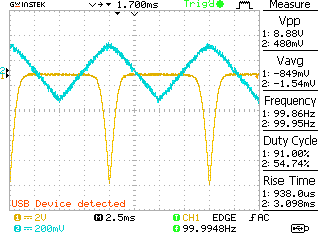
\includegraphics[width=0.7\textwidth]{../data/DS0000.png}
    \captionof{figure}{Inverted Exponentiater oscillogramm}
    \label{fig:invexpoisc}
	\end{Figure}
  Here we can observe the exponential-like amplification for positiv voltages.
        \subsection{Non--inverting exponentiator}
        \begin{Figure}
                \centering
                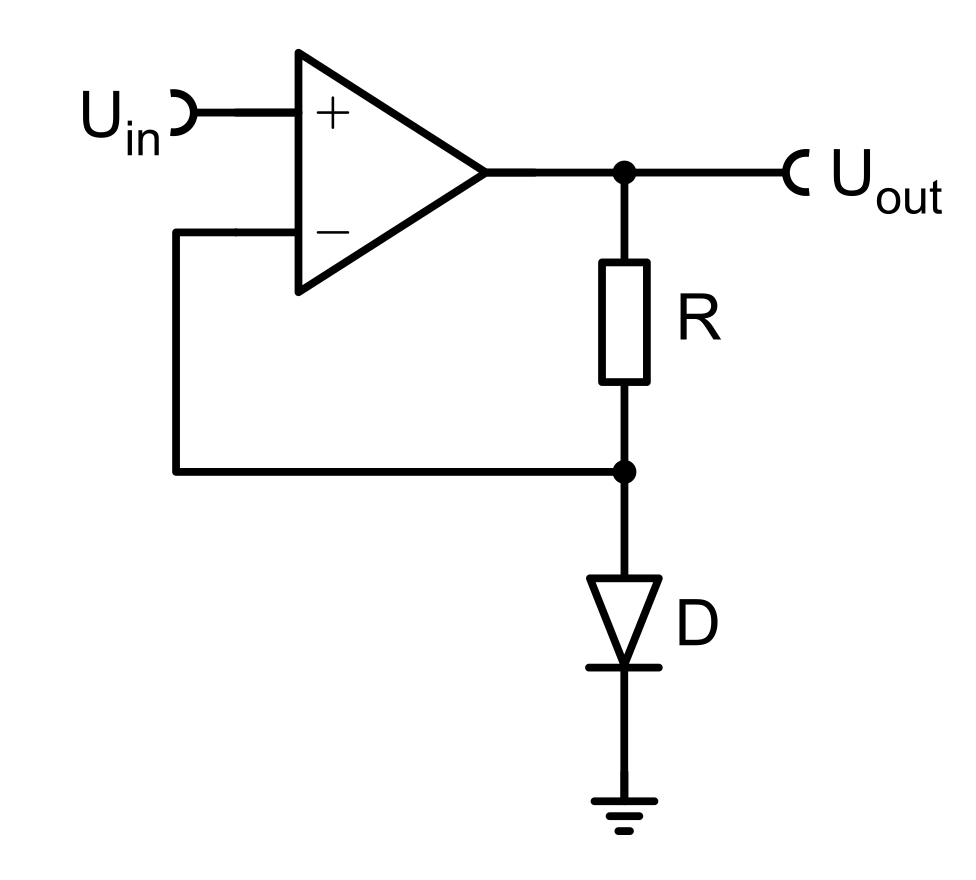
\includegraphics[width=0.6\textwidth]{non_inverting_exp.png} \label{fig:non_inverting_exp}
                \captionof{figure}{Non--inverting exponentiator; Abb.\ 6.5\cite{Praktikumsanleitung}}
        \end{Figure}
        The input impedance of the non--inverting exponentiator is very high, because the opamp has a high input impedance.
        The output voltage of this circuit can be calculated via the golden rules (g.r.) of an opamp.
        \textsc{Kirchhoff}s law states that
        \begin{align} 
                 &&&& I_D &= I_R+I_- &&&& \,|\, \text{g.r. }I_-=0\\
                 \Leftrightarrow  &&&& I_D &= I_R &&&& \\
                 \Leftrightarrow  &&&& I_D &= \dfrac{U_R}{R} &&&& \,|\, U_R=U_\text{out}-\underbrace{U_-}_{U_\text{in}}\\
                 \Leftrightarrow  &&&& I_D &= \dfrac{U_\text{out}-U_\text{in}}{R} &&&& \,|\, I_D=I_0\text{e}^{\alpha U_\text{in}}\\
                 \Leftrightarrow  &&&& RI_0\text{e}^{\alpha U_\text{in}} &= U_\text{out}-U_\text{in} &&&& \,|\, A:=RI_0,B:=\dfrac{1}{\alpha }\\
                 \Leftrightarrow  &&&& U_\text{out} &= A\text{e}^{\tfrac{U_\text{in}}{B}}+U_\text{in} &&&& 
        \end{align} 
        The ciruit \ref{fig:non_inverting_exp} is built with $R=\SI{47}{k\ohm}$ and a Si--diode. 
        The input is a triangle signal.
        The signal is amplified solely when the polarity is aligned with that of the diode, the other polarity is not amplified.
        Because the signal is alternating current, the diode behaves differently for different polarity.
        Forward bias: 
        When in forward bias the signal gets amplified exponentially, when the threshold voltage is reached.
        This happenes because the feedback current is routed into ground by the low impedance of the diode, thus it is not regulating the opamp resulting in an exponential gain.
        Reverse bias: 
        In Reverse bias the diode has a very high impedance, which means, the current from the feedback loop is completely fed into the opamp.
        This results in no amplification of the input signal.
        Because the output voltage also has a linear term, the input voltage is mimicked.
        The same happenes for very low input voltages, i.e.\ when the signal passes zero or is lower than one, because the exponential term doesn't contribute.
        After an input voltage of one, the output starts to rise exponentially.
        When the input is too large, the opamp gets saturated and maxes out at the supply voltage.\par
        The next part is done with a \textsc{Schottky}diode.
        A \textsc{Schottky}diode has a lower forward bias than the Si--diode, which means that the signal will be amplified for lower input voltages.
        Also, the \textsc{Schottky}diode has a current running in reverse bias which is considerably more, than the Si--diode has.
        This results in the output voltage (which is still mimicked by the linear term) to be amplified by this reverse current.
        \begin{Figure}
                \centering
                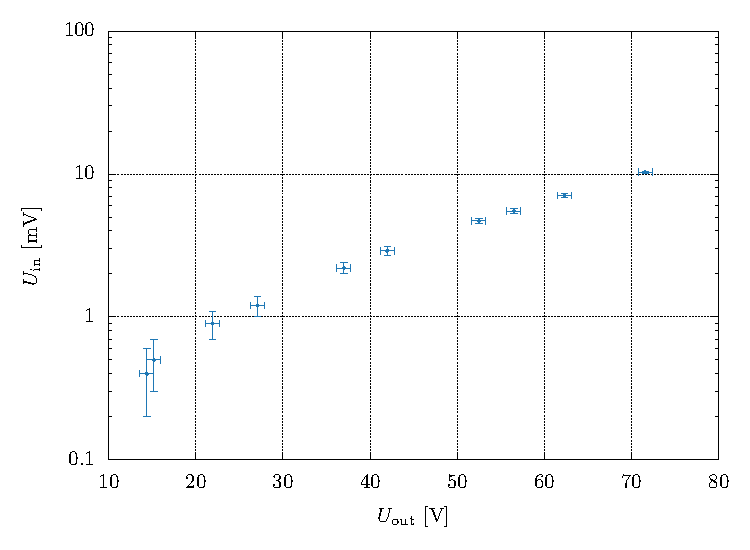
\includegraphics[width=0.6\textwidth]{../plot/6_1_2_crop.pdf}
                \captionof{figure}{$U_\text{in}$--$U_\text{out}$--diagram of the non--inverting amplifier (\textsc{Schottky}diode)}
        \end{Figure}
        \noindent One can see, that the amplification is exponential (linear in this log plot).
        The amplification for low input signals is not as steep, due to the UI--curve of the \textsc{Schottky}diode.
        This behavior was expected because the circuit amplifies a signal exponentially.


  \subsection{The grand circuit}
  After we have assambled our non-inverting exponentiater with a potentiometer we plug the Sawtooth-Generator infront of our circuit and plug our circuit in the voltage-fequency-changer. After some debugging we hear a singal from the speaker thats pluged into the the voltage-frequency-changer. Todays lab course was a very pleasend one, since in comparisson to the last ones we had not to do as meany meassuremnts or analysis. It was a nice experimente to see the diffrent use cases for an op amp.
  \section{Conclusion}
  In the lab course we constructed a inverting and non-inverting exponentiater with diffrent resistors and a potantiometer. We saw from fig. \ref{fig:invexpoisc} the amplification with an exponential behaviour.

  At the end we connected all the diffrent kinds of circuits to achieve a sound from a speaker connected at the end. 
\end{multicols}

\clearpage
\listoffigures
\listoftables
\bibliographystyle{plain}
\bibliography{refs}

%}}}

\end{document}
